\newpage
\section{Arithmetik}
	
	\begin{multicols}{2}
		\subsection{1er-Komplement}
			\[
				\langle s_nd_{n-1} \ldots d_0 \rangle_{1er} := \begin{cases}
				\sum\limits_{i=0}^{n-1} d_i \cdot 2^i          &  s_n = 0\\
				-\sum\limits_{i=0}^{n-1} (1-d_i) \cdot 2^i     & s_n = 1 
				\end{cases}
			\]
			
		\subsection{Sign magnitude}
		Uses the most significant bit to show if value is positive or negative, 0 positive and 1 negative. But addition doesn't work and two zeros
		
		\subsection{2er-Komplement}
		To go from one to the other you invert the bits and add 1. Watch out because doing addition, if there are not enough bits the addition can overflow making a negative number where there shouldn't be one.
			\begin{align*}
				[\![ s_nd_{n-1} \ldots d_0 ]\!] &= \begin{cases}
				\sum\limits_{i=0}^{n-1} d_i \cdot 2^i          &  s_n = 0\\
				-(1 + \sum\limits_{i=0}^{n-1} (1-d_i) \cdot 2^i)     & s_n = 1 
				\end{cases} \\
				& =  s_n \cdot -2^n + \sum \limits_{i=0}^{n-1} d_i \cdot 2^i
			\end{align*}

		\subsection{Lemma}
			\[ 2^n = 1 + \sum\limits_{i=0}^{n-1} 1 \cdot 2^i \]
	\end{multicols}
	\subsection{Number systems}
	\paragraph{Fixed point numbers}, are a representation of a fraction, they have a point somewhere in the number and after the point the exponent becomes negative. Two's complement works with fixed point numbers.
	\begin{equation}
		01101100 = 2^2+2^1+2^-1+2^-2 = 6.75
	\end{equation}
	\paragraph{Floating point}, are like a scientific representation, they have a mantissa(M), a base(B) and an exponent(E). 32 bits are used, 1 for the sign, 23 for the mantissa and 8 for the exponent.

	
	\vspace{8mm}
	\subsection{Operations}
	
	\begin{multicols}{2}
		\subsubsection{Halbaddierer}
			\begin{tabular}{r@{\quad$\equiv$\quad}l@{\quad$\equiv$\quad}l}
				$s$ & $(a + b) \text{ mod } 2$ & $a \oplus b$ \\
				$o$ & $(a + b) \text{ div } 2$ & $a \land b$ \\
			\end{tabular}
		
		\subsubsection{Volladdierer}
			\begin{tabular}{r@{\quad$\equiv$\quad}l@{\quad$\equiv$\quad}l}
				$s$ & $(a + b + i) \text{ mod } 2$ & $a \oplus b \oplus i $ \\
				$o$ & $(a + b + i) \text{ div } 2$ & $ a \cdot b + a \cdot i + b \cdot i$ \\
			\end{tabular}
			
		\subsubsection{Überlauf}
		\[ [\![a]\!] + [\![b]\!] \notin \{-2^{n-1}, \ldots, 2^{n-1}-1\} \quad \iff \quad c_{n-1} \oplus c_n \]
			
		\subsubsection{Ripple-Carry Addierer}
		Einfacher Addierer mit $O(n)$ Zeit und Platz.
			\begin{center}
			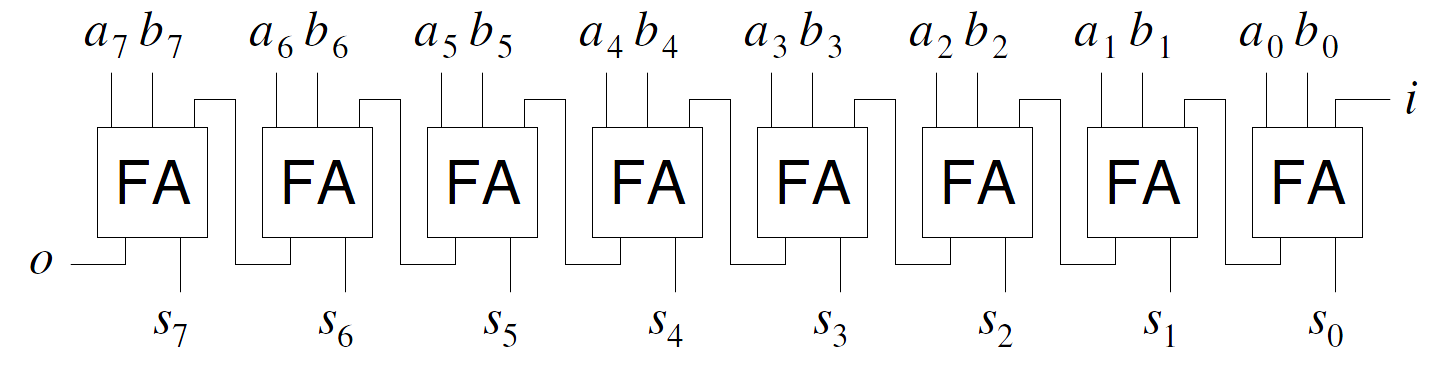
\includegraphics[width = 9cm]{images/arith/ripple.png}
			\end{center}
		
	\end{multicols}
	
	\vspace{8mm}
	
	\subsubsection{Booth Recoding - Multiplikation zweier Binärzahlen ($A \cdot B$)}
	\begin{multicols}{2}
		
			\begin{enumerate}
				\item Wähle kürzere der beiden Zahlen als $A$, wähle $P$ gleich lang wie $B$\\[-5mm]
				\item Erstelle Tabelle $P_{m, \ldots, 0} \mid A_{n, \ldots, 0} \mid A_{-1}$ = 0\\[-5mm]
				\item Wende folgende \emph{Regeln} an, starte bei $i = 0$, Tue bei jedem Schritt: $i := i + 1$:\\[1.5mm]
					\begin{tabular}{l | l | l}
						$A_i$   &   $A_{i-1}$   &   ToDo\\\hline\hline
						0       &   0           &   - \\\hline
						0       &   1           &   addiere B zu P\\\hline
						1       &   0           &   addiere -B zu P\\\hline
						1       &   1           &   -
					\end{tabular}
					\\[-2mm]
				\item Shifte arithmetisch nach rechts (d.h. Vorzeichen nachschieben)\\[-5.5mm]
				\item Wiederhole (3) und (4) $n$ (Länge A) mal\\[-5.5mm]
			\end{enumerate}
			
		\columnbreak
		
			\begin{center}
			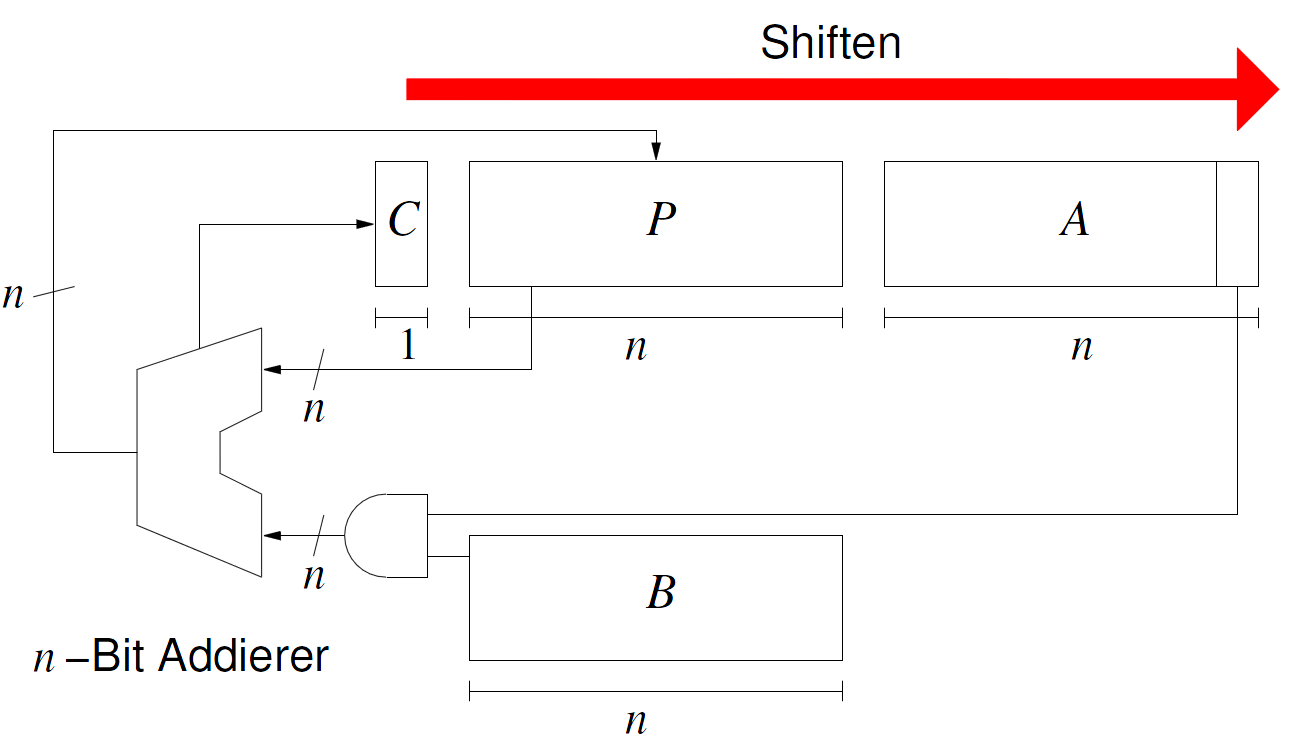
\includegraphics[width = 7cm]{images/arith/mult.png}
			\end{center}
	\end{multicols}

		
		
		
		
		
		
		
		
		
		
		
		
		
		
		
		
		
		
		
		
		
		
		